% Figure source (pretrain). Rendered to figures/pdf/pretrain.pdf by the
% figure build; delete that PDF to have LaTeX compile this source instead.
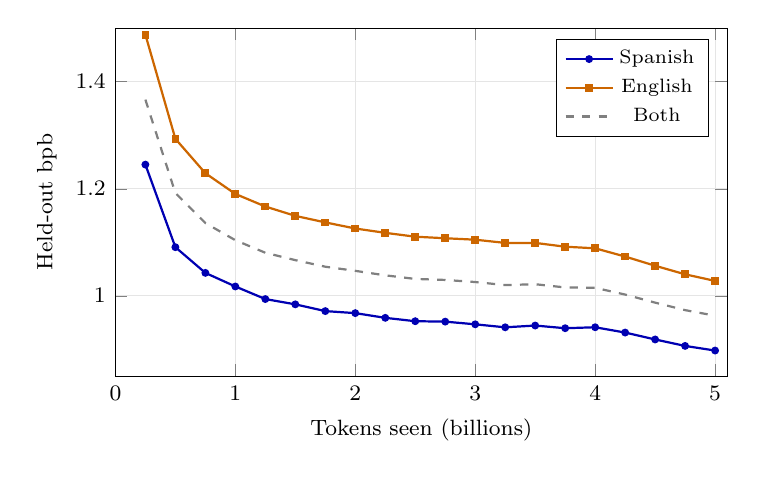
\begin{tikzpicture}
\begin{axis}[
    width=9.35cm, height=6cm,
    xlabel={Tokens seen (billions)}, ylabel={Held-out bpb},
    xmin=0, xmax=5.1, ymin=0.85, ymax=1.5,
    legend pos=north east, legend style={font=\scriptsize},
    tick label style={font=\footnotesize}, label style={font=\footnotesize},
    grid=major, grid style={gray!20}
]
\addplot[blue!70!black, thick, mark=*, mark size=1pt] coordinates {
 (0.25,1.2452) (0.5,1.0909) (0.75,1.0429) (1.0,1.0175) (1.25,0.994) (1.5,0.9841) (1.75,0.9715) (2.0,0.9677) (2.25,0.9589) (2.5,0.9526) (2.75,0.9518) (3.0,0.9468) (3.25,0.9412) (3.5,0.9445) (3.75,0.9395) (4.0,0.9413) (4.25,0.9314) (4.5,0.9185) (4.75,0.9064) (5.0,0.8978)};
\addlegendentry{Spanish}
\addplot[orange!80!black, thick, mark=square*, mark size=1pt] coordinates {
 (0.25,1.488) (0.5,1.2934) (0.75,1.2291) (1.0,1.1904) (1.25,1.1669) (1.5,1.1494) (1.75,1.1372) (2.0,1.1258) (2.25,1.1177) (2.5,1.1105) (2.75,1.1076) (3.0,1.1049) (3.25,1.0989) (3.5,1.0989) (3.75,1.0918) (4.0,1.0888) (4.25,1.0734) (4.5,1.0562) (4.75,1.0402) (5.0,1.0279)};
\addlegendentry{English}
\addplot[gray, thick, dashed] coordinates {
 (0.25,1.3666) (0.5,1.1921) (0.75,1.136) (1.0,1.1039) (1.25,1.0805) (1.5,1.0667) (1.75,1.0544) (2.0,1.0467) (2.25,1.0383) (2.5,1.0316) (2.75,1.0297) (3.0,1.0258) (3.25,1.0201) (3.5,1.0217) (3.75,1.0157) (4.0,1.015) (4.25,1.0024) (4.5,0.9873) (4.75,0.9733) (5.0,0.9629)};
\addlegendentry{Both}
\end{axis}
\end{tikzpicture}
